\documentclass[10pt,aspectratio=169]{beamer}

\usetheme{Madrid}
\usecolortheme{default}
\setbeamertemplate{navigation symbols}{}
\setbeamertemplate{footline}[frame number]

\usepackage{booktabs}
\usepackage{array}
\usepackage{amsmath}
\usepackage{multirow}
\usepackage{xcolor}
\usepackage{graphicx}
\usepackage{tikz}
\usetikzlibrary{arrows.meta,positioning}

\definecolor{mainblue}{RGB}{36,82,140}
\definecolor{accent}{RGB}{0,128,128}
\definecolor{softgray}{RGB}{245,247,250}

\setbeamercolor{structure}{fg=mainblue}
\setbeamercolor{frametitle}{fg=white,bg=mainblue}
\setbeamercolor{title}{fg=white,bg=mainblue}
\setbeamercolor{block title}{fg=white,bg=mainblue}
\setbeamercolor{block body}{bg=softgray}

\title[EEG Classification]{EEG-Based Epileptic Signal Classification Using Bayesian-Optimized SVM}
\author{Your Name}
\institute{Final Year Project}
\date{\today}

\begin{document}

\begin{frame}
  \titlepage
\end{frame}

\begin{frame}{Presentation Outline}
  \tableofcontents
\end{frame}

\section{Background and Dataset}

\begin{frame}{Background}
  \begin{itemize}
    \item Epilepsy is a neurological disorder characterized by abnormal brain activity.
    \item Electroencephalography (EEG) directly records brain electrical signals and is widely used for epilepsy analysis.
    \item Automatic EEG classification can reduce manual workload and support clinical decision-making.
  \end{itemize}

  \begin{block}{Project Focus}
    This project develops a feature-based RBF-SVM pipeline for Bonn EEG classification and improves it using Bayesian Optimization.
  \end{block}
\end{frame}

\begin{frame}{Bonn EEG Dataset}
  \begin{itemize}
    \item Dataset: University of Bonn EEG dataset.
    \item Five sets, 100 EEG segments per set.
    \item Sampling frequency: 173.61 Hz; each segment contains 4097 samples.
    \item In this project, the dataset is treated as five classes: Z, O, N, F, and S.
  \end{itemize}

  \begin{table}
    \centering
    \scriptsize
    \resizebox{\textwidth}{!}{%
    \begin{tabular}{lllp{5.4cm}}
      \toprule
      Z & Z000--Z100.txt & 564 KB & Five healthy subjects with open eyes \\
      O & O000--O100.txt & 611 KB & Five healthy subjects with closed eyes \\
      N & N000--N100.txt & 560 KB & Five people with epilepsy in seizure-free status \\
      F & F000--F100.txt & 569 KB & Five people with epilepsy in seizure-free status inside epileptogenic zones \\
      S & S000--S100.txt & 747 KB & Five subjects during seizure activity \\
      \bottomrule
    \end{tabular}
    }
  \end{table}

  \begin{block}{Notation Used in This Project}
    The original Bonn dataset is often described as Set A--E. In this project, the classification labels are reported directly as Z, O, N, F, and S.
  \end{block}
\end{frame}

\begin{frame}{Project Objectives}
  \begin{enumerate}
    \item Build a complete EEG classification pipeline for the Bonn dataset.
    \item Compare standard SVM, Bayesian-Optimized SVM, and Random Search SVM.
    \item Analyze classification errors using recall and confusion matrices.
    \item Improve five-class performance by tuning preprocessing and SVM hyperparameters.
    \item Evaluate both five-class and binary/three-class subset tasks.
  \end{enumerate}
\end{frame}

\section{Methodology}

\begin{frame}{Overall Pipeline}
  \centering
  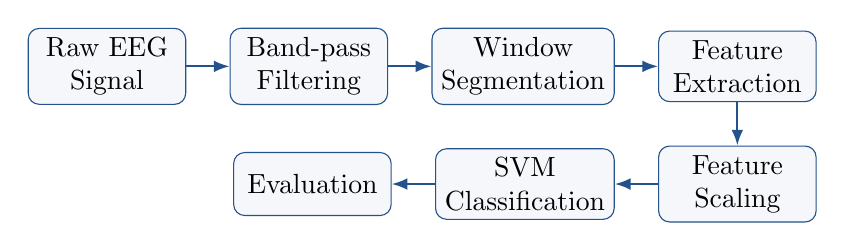
\begin{tikzpicture}[
    node distance=0.55cm,
    box/.style={draw=mainblue, rounded corners, align=center, minimum width=2.0cm, minimum height=0.8cm, fill=softgray},
    arrow/.style={-{Latex[length=2mm]}, thick, mainblue}
  ]
    \node[box] (raw) {Raw EEG\\Signal};
    \node[box, right=of raw] (filter) {Band-pass\\Filtering};
    \node[box, right=of filter] (window) {Window\\Segmentation};
    \node[box, right=of window] (features) {Feature\\Extraction};
    \node[box, below=of features] (scale) {Feature\\Scaling};
    \node[box, left=of scale] (svm) {SVM\\Classification};
    \node[box, left=of svm] (eval) {Evaluation};

    \draw[arrow] (raw) -- (filter);
    \draw[arrow] (filter) -- (window);
    \draw[arrow] (window) -- (features);
    \draw[arrow] (features) -- (scale);
    \draw[arrow] (scale) -- (svm);
    \draw[arrow] (svm) -- (eval);
  \end{tikzpicture}

  \vspace{0.5cm}
  \begin{block}{Main Idea}
    EEG windows are converted into feature vectors, then classified using RBF-SVM.
  \end{block}
\end{frame}

\begin{frame}{Signal Preprocessing}
  \begin{itemize}
    \item Band-pass filtering was used to retain useful EEG frequency components.
    \item EEG segments were divided into fixed-length windows.
    \item Both non-overlapping and 50\% overlapping windows were tested.
    \item Overlap was added as a Bayesian Optimization search parameter.
  \end{itemize}

  \begin{block}{Important Evaluation Note}
    Overlapping windows increase the number of EEG windows before train/validation/test splitting, so the result should be reported as window-level performance.
  \end{block}
\end{frame}

\begin{frame}{Feature Extraction}
  \begin{columns}
    \begin{column}{0.50\textwidth}
      \begin{block}{Frequency-Domain Features}
        \begin{itemize}
          \item PSD band power
          \item Relative band power
        \end{itemize}
      \end{block}

      \begin{block}{Statistical Features}
        \begin{itemize}
          \item Mean, variance, standard deviation
          \item RMS, line length
          \item Skewness and kurtosis
        \end{itemize}
      \end{block}
    \end{column}

    \begin{column}{0.46\textwidth}
      \begin{block}{Nonlinear Features}
        \begin{itemize}
          \item Shannon entropy
          \item Spectral entropy
          \item Approximate entropy
          \item Hjorth parameters
        \end{itemize}
      \end{block}

      \begin{block}{Fixed Feature Setting}
        \begin{itemize}
          \item PSD/statistical features
          \item Entropy features
          \item Hjorth features
        \end{itemize}
      \end{block}
    \end{column}
  \end{columns}
\end{frame}

\begin{frame}{PSD Normalization}
  \begin{itemize}
    \item Power Spectral Density (PSD) describes how signal power is distributed across frequencies.
    \item Absolute band power can be affected by overall signal amplitude.
    \item Therefore, relative band power was computed:
  \end{itemize}

  \[
    \text{Relative Power}_{i} =
    \frac{\text{Band Power}_{i}}
    {\sum_{j=1}^{5}\text{Band Power}_{j}}
  \]

  \begin{block}{Purpose}
    PSD normalization makes samples more comparable and helps the model focus on frequency distribution rather than absolute signal magnitude.
  \end{block}
\end{frame}

\begin{frame}{Bayesian Optimization Objective}
  \begin{itemize}
    \item Bayesian Optimization was used to search preprocessing and SVM hyperparameters.
    \item The main five-class BO-SVM experiment was run for 80 iterations.
    \item The feature setting was fixed to keep the method clear and reproducible.
  \end{itemize}

  \[
    \text{Score} =
    0.35\,\text{Accuracy}
    + 0.25\,\text{Macro Recall}
    + 0.20\,\text{Recall}_{N}
    + 0.20\,\text{Recall}_{F}
  \]

  \begin{block}{Reason for N/F Weighting}
    Earlier confusion matrices showed that N and F were the most difficult classes to separate.
  \end{block}
\end{frame}

\section{BO-SVM Baseline}

\begin{frame}{BO-SVM Baseline}
  \begin{itemize}
    \item RBF-SVM was selected as the base classifier.
    \item SVM is suitable for small datasets and handcrafted high-dimensional features.
    \item Bayesian Optimization was used to tune important hyperparameters.
  \end{itemize}

  \begin{table}
    \centering
    \small
    \begin{tabular}{ll}
      \toprule
      Parameter & Meaning \\
      \midrule
      $f_{low}$, $f_{high}$ & Band-pass frequency range \\
      Window size & EEG window length \\
      Overlap & Non-overlap or 50\% overlap \\
      $C$ & SVM regularization parameter \\
      $\gamma$ & RBF kernel parameter \\
      \bottomrule
    \end{tabular}
  \end{table}

  \begin{block}{Fixed Settings}
    Feature setting = entropy\_hjorth, class\_weight = balanced.
  \end{block}
\end{frame}

\begin{frame}{Baseline Finding}
  \begin{itemize}
    \item The initial BO-SVM achieved around 84--86\% test accuracy.
    \item Confusion matrix analysis showed that the seizure class S was detected very well.
    \item Most remaining errors came from confusion between N and F.
  \end{itemize}

  \begin{block}{Key Observation}
    The main problem was not seizure detection, but separating similar interictal EEG classes N and F.
  \end{block}
\end{frame}

\section{BO-SVM Optimization}

\begin{frame}{Bayesian Optimization Workflow}
  \centering
  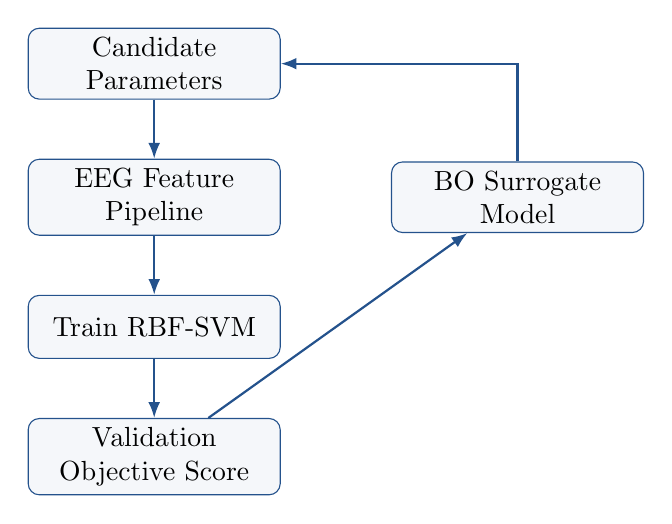
\begin{tikzpicture}[
    node distance=0.75cm,
    box/.style={draw=mainblue, rounded corners, align=center, minimum width=3.2cm, minimum height=0.8cm, fill=softgray},
    arrow/.style={-{Latex[length=2mm]}, thick, mainblue}
  ]
    \node[box] (params) {Candidate\\Parameters};
    \node[box, below=of params] (pipeline) {EEG Feature\\Pipeline};
    \node[box, below=of pipeline] (svm) {Train RBF-SVM};
    \node[box, below=of svm] (score) {Validation\\Objective Score};
    \node[box, right=1.4cm of pipeline] (bo) {BO Surrogate\\Model};

    \draw[arrow] (params) -- (pipeline);
    \draw[arrow] (pipeline) -- (svm);
    \draw[arrow] (svm) -- (score);
    \draw[arrow] (score) -- (bo);
    \draw[arrow] (bo) |- (params);
  \end{tikzpicture}

  \vspace{0.35cm}
  \begin{block}{Motivation}
    BO uses previous evaluations to choose the next parameter setting more efficiently than random trial-and-error.
  \end{block}
\end{frame}

\begin{frame}{Final BO-SVM Setting}
  \begin{table}
    \centering
    \small
    \begin{tabular}{ll}
      \toprule
      Component & Setting \\
      \midrule
      Classifier & RBF-SVM \\
      Feature setting & entropy\_hjorth \\
      Class weighting & balanced \\
      BO iterations & 80 \\
      Search parameters & $f_{low}$, $f_{high}$, window size, overlap, $C$, $\gamma$ \\
      Comparison methods & Manual SVM and Random Search SVM \\
      \bottomrule
    \end{tabular}
  \end{table}
\end{frame}

\section{Results}

\begin{frame}{Five-Class Classification Results}
  \begin{table}
    \centering
    \begin{tabular}{lc}
      \toprule
      Method & Test Accuracy \\
      \midrule
      SVM without BO & 76.45\% \\
      Random Search SVM & 84.25\% \\
      SVM with BO & \textbf{86.00\%} \\
      \bottomrule
    \end{tabular}
  \end{table}

  \begin{block}{Interpretation}
    BO-SVM achieved the best five-class test accuracy and improved over both manual SVM and random search.
  \end{block}
\end{frame}

\begin{frame}{Main Result Visualization}
  \begin{columns}
    \begin{column}{0.48\textwidth}
      \centering
      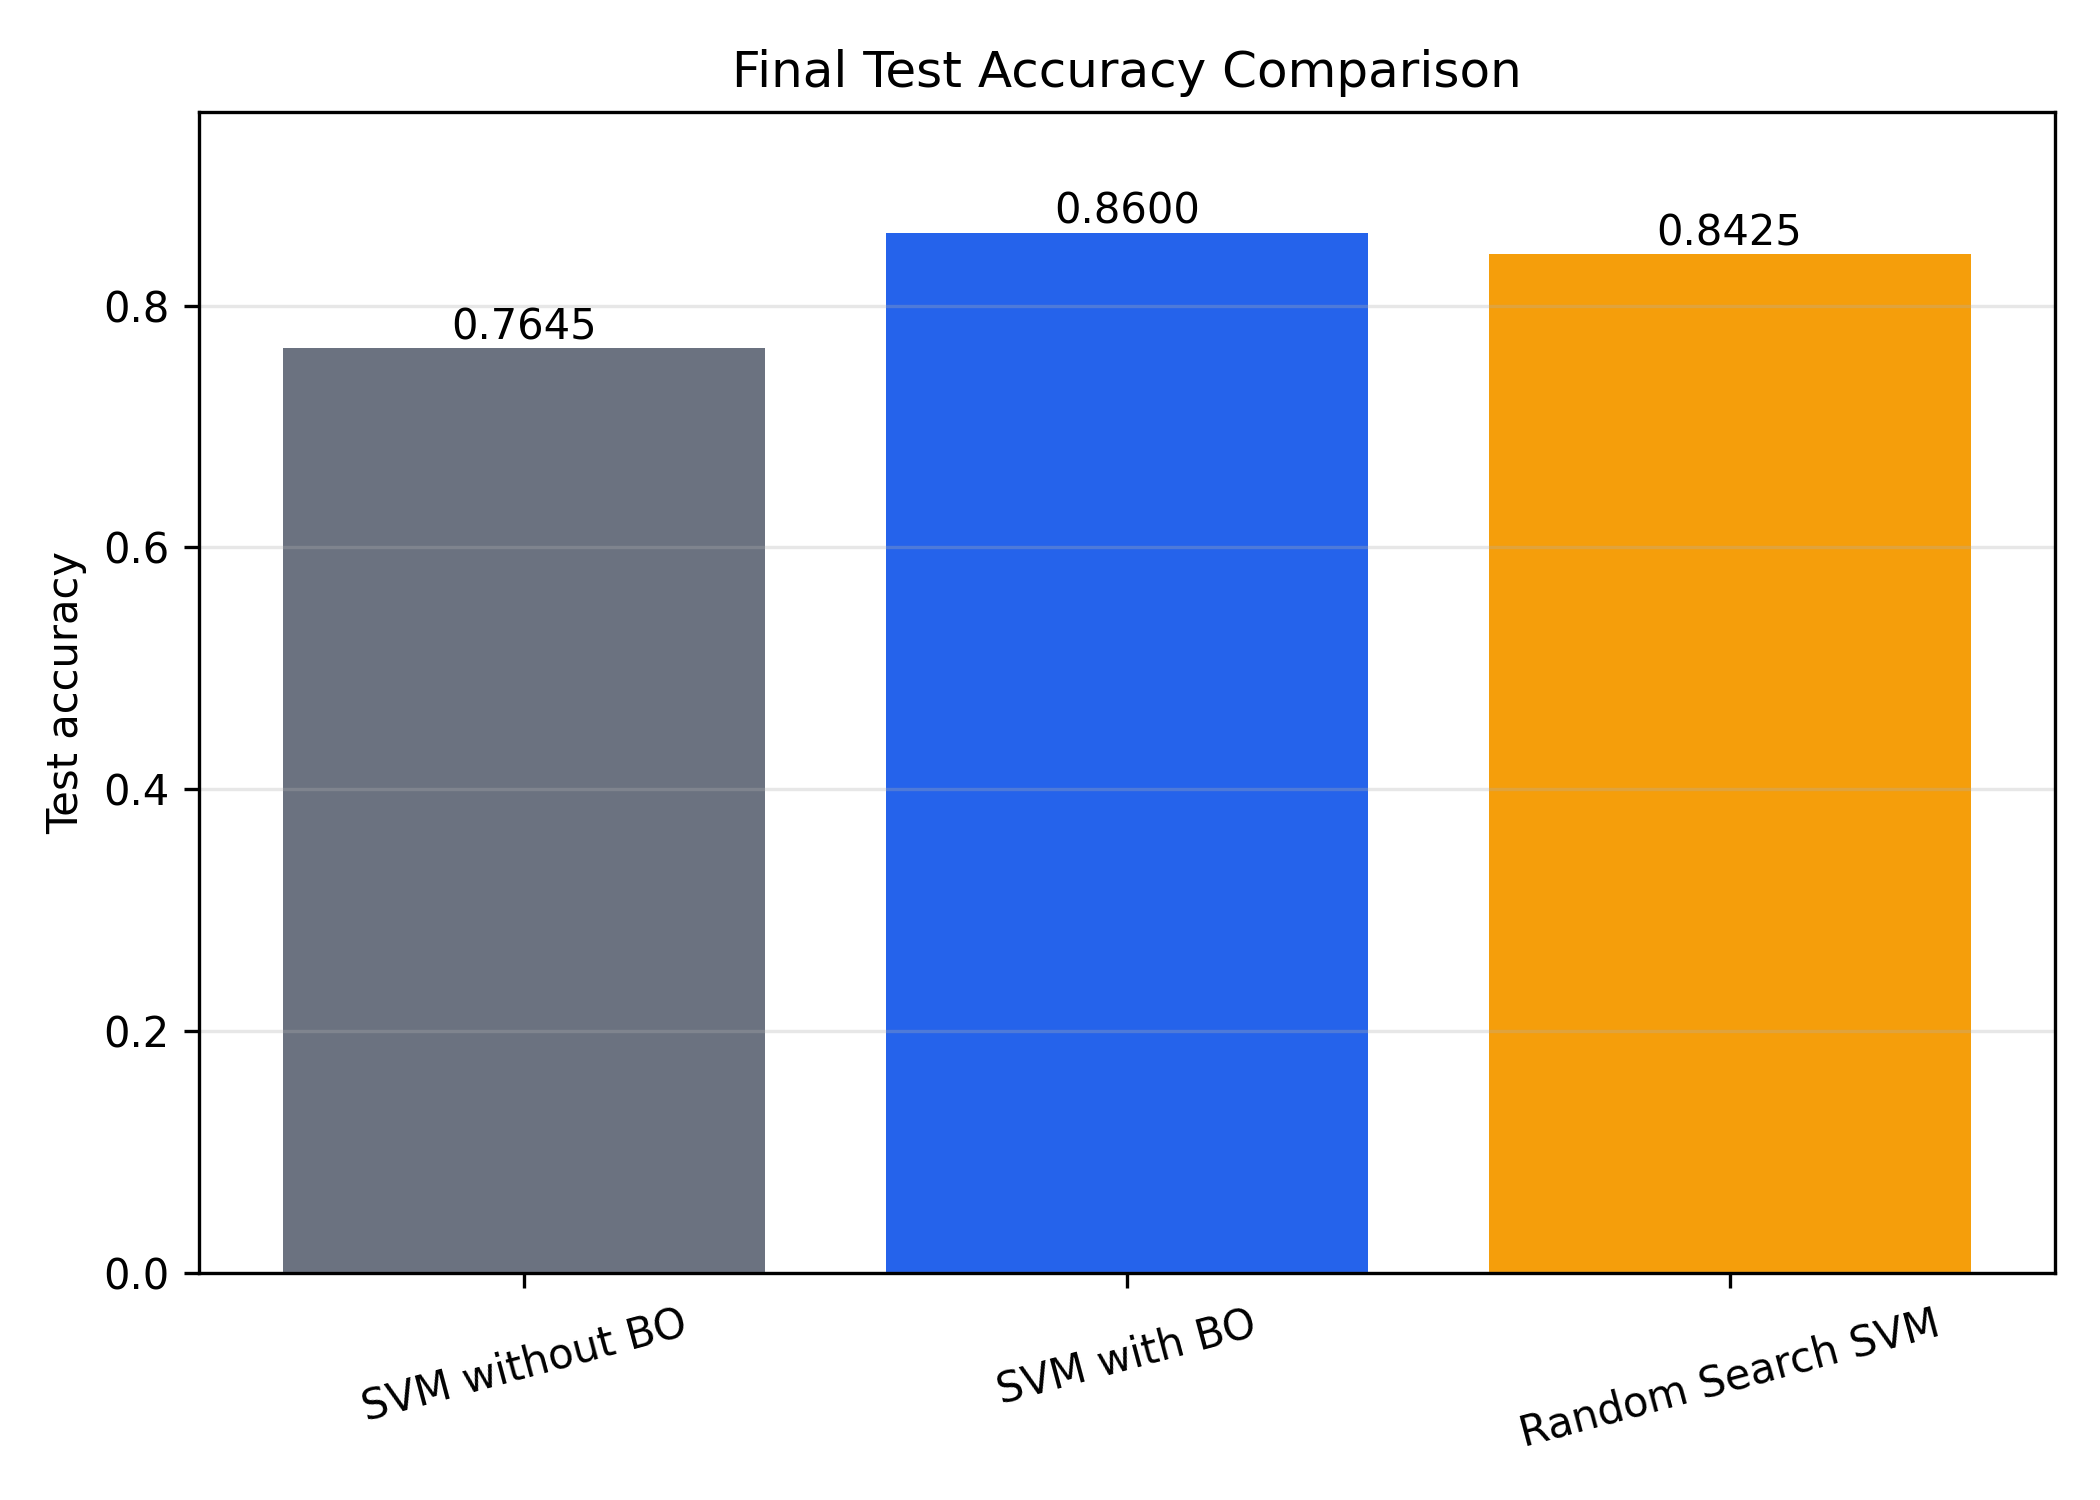
\includegraphics[width=\textwidth]{results/00_main_bo_svm/test_accuracy_comparison.png}

      \vspace{0.1cm}
      \scriptsize Final test accuracy comparison
    \end{column}

    \begin{column}{0.48\textwidth}
      \centering
      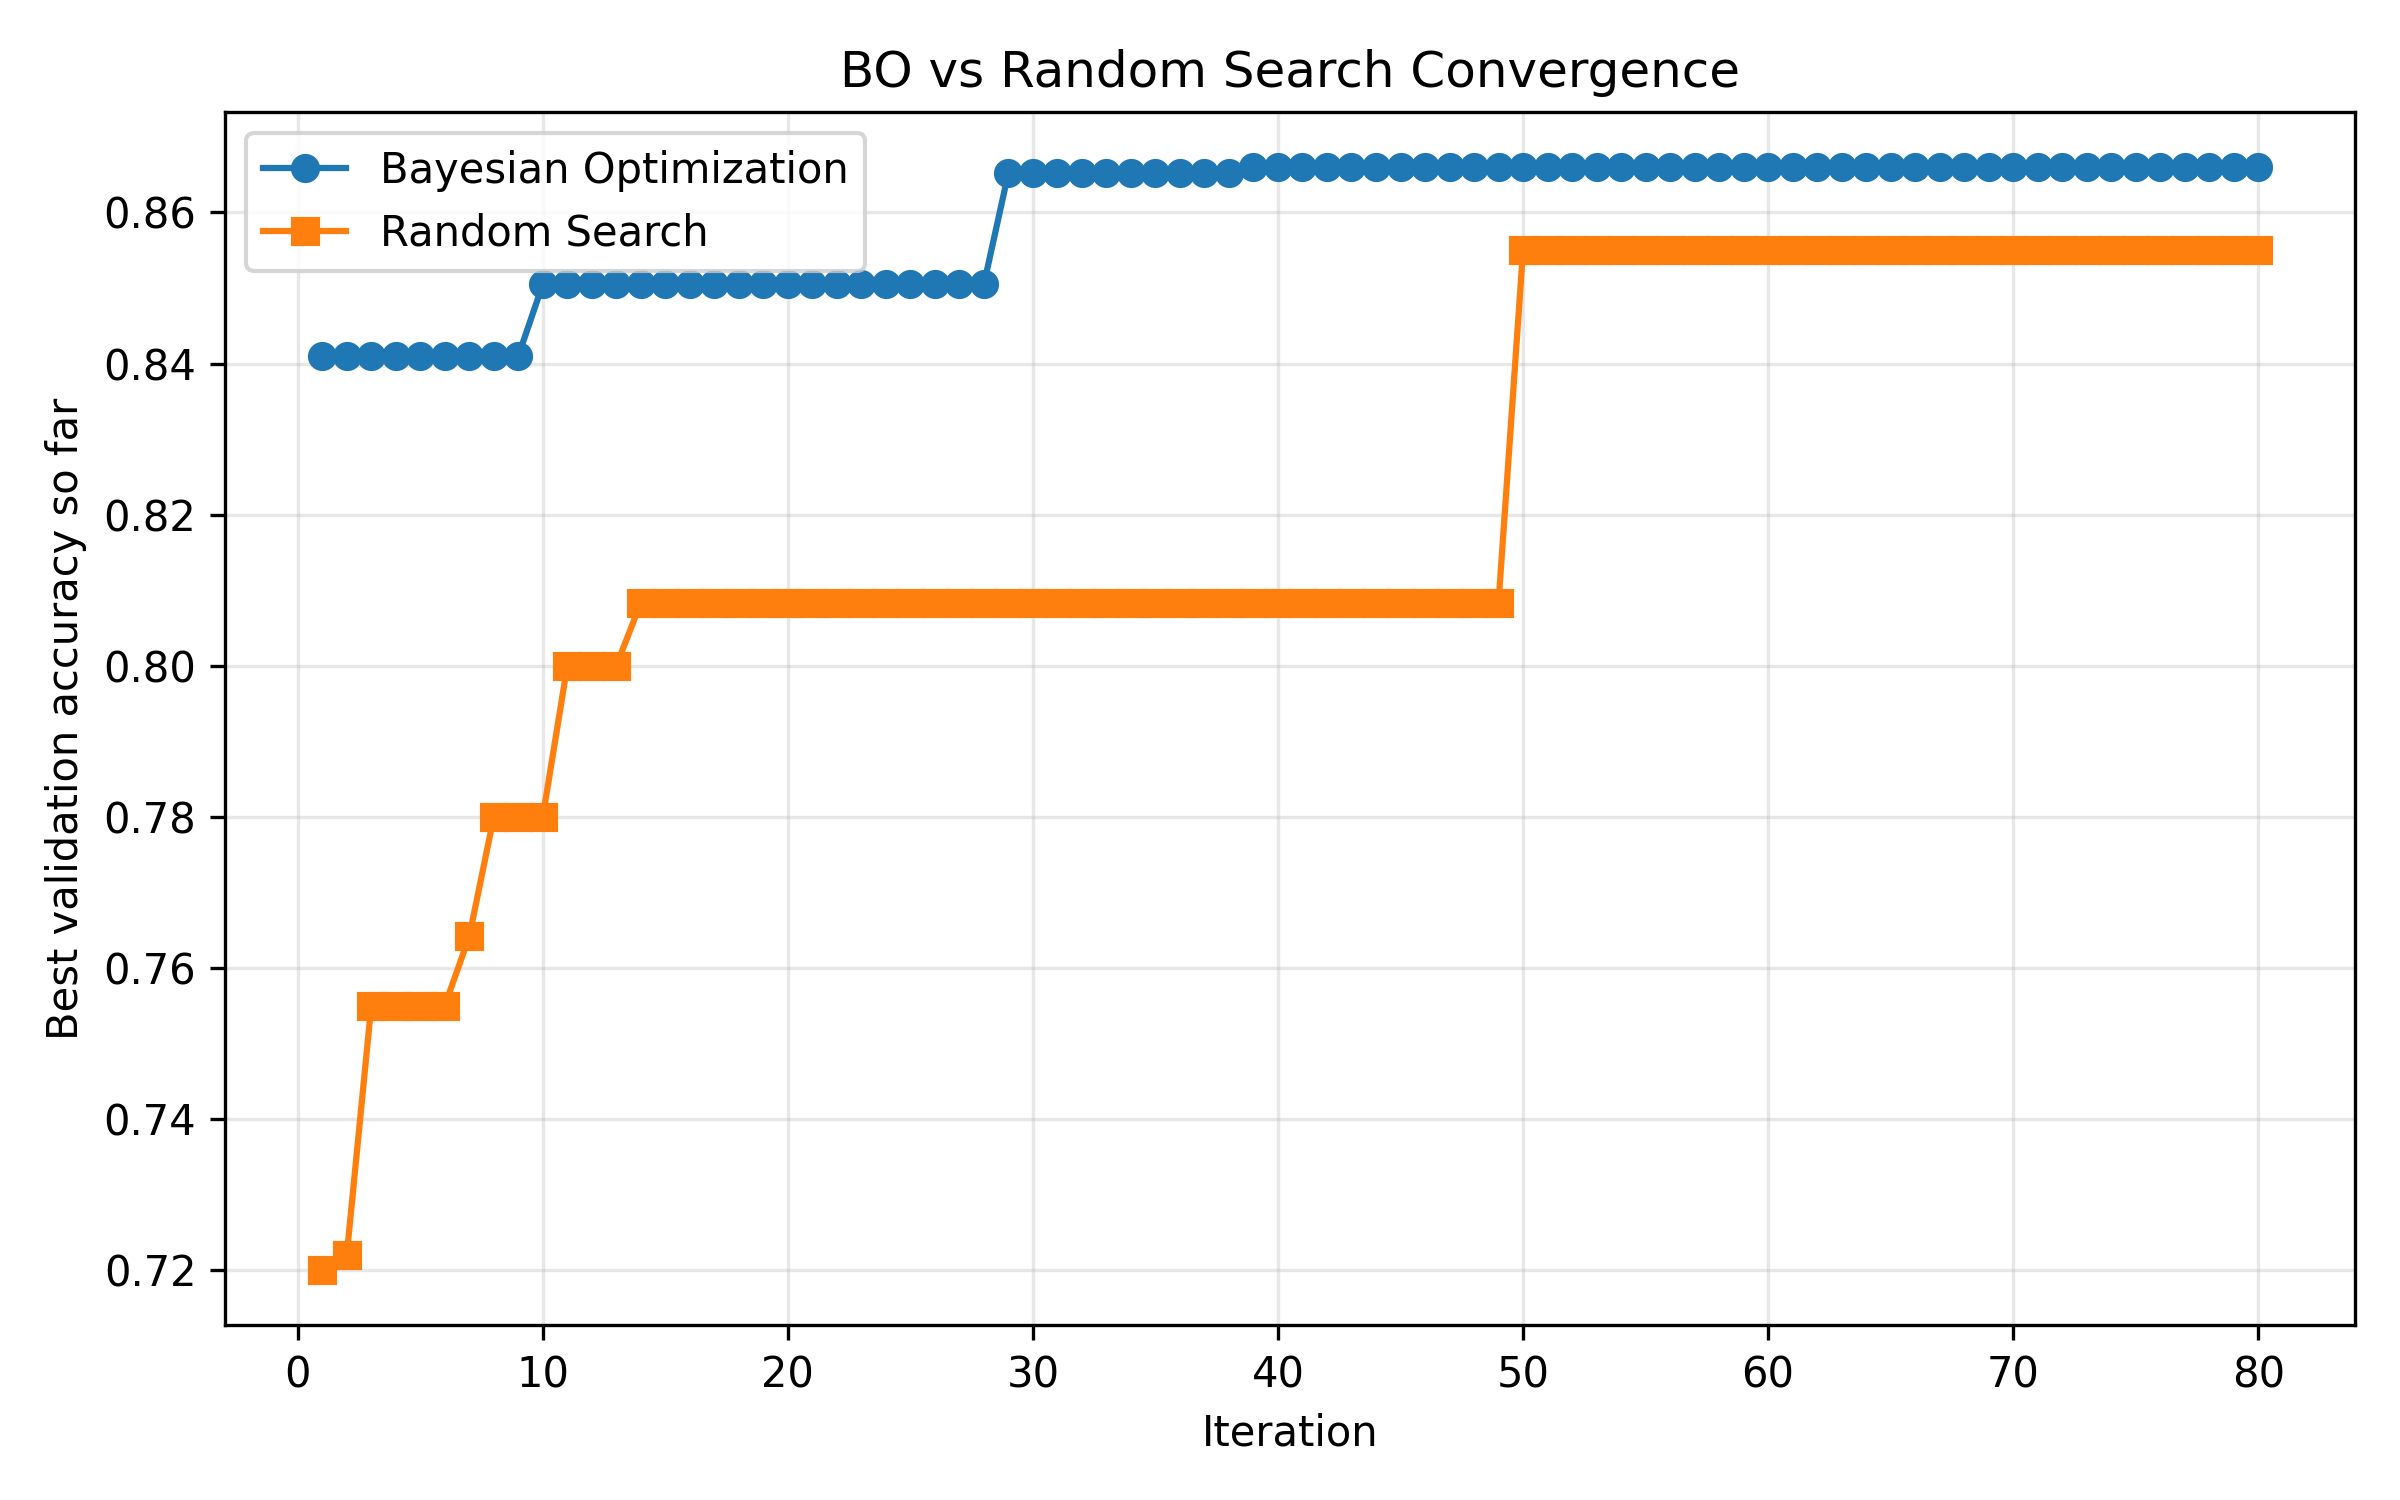
\includegraphics[width=\textwidth]{results/00_main_bo_svm/convergence_bo_vs_random.png}

      \vspace{0.1cm}
      \scriptsize BO vs Random Search convergence
    \end{column}
  \end{columns}
\end{frame}

\begin{frame}{Best Five-Class BO-SVM Result}
  \begin{table}
    \centering
    \small
    \begin{tabular}{lc}
      \toprule
      Metric & Value \\
      \midrule
      Test accuracy & \textbf{86.00\%} \\
      Macro recall & \textbf{86.00\%} \\
      Recall Z & 93.12\% \\
      Recall O & 84.38\% \\
      Recall N & 86.88\% \\
      Recall F & 66.25\% \\
      Recall S & 99.38\% \\
      \bottomrule
    \end{tabular}
  \end{table}
\end{frame}

\begin{frame}{Five-Class Recall and Confusion Matrix}
  \begin{columns}
    \begin{column}{0.48\textwidth}
      \centering
      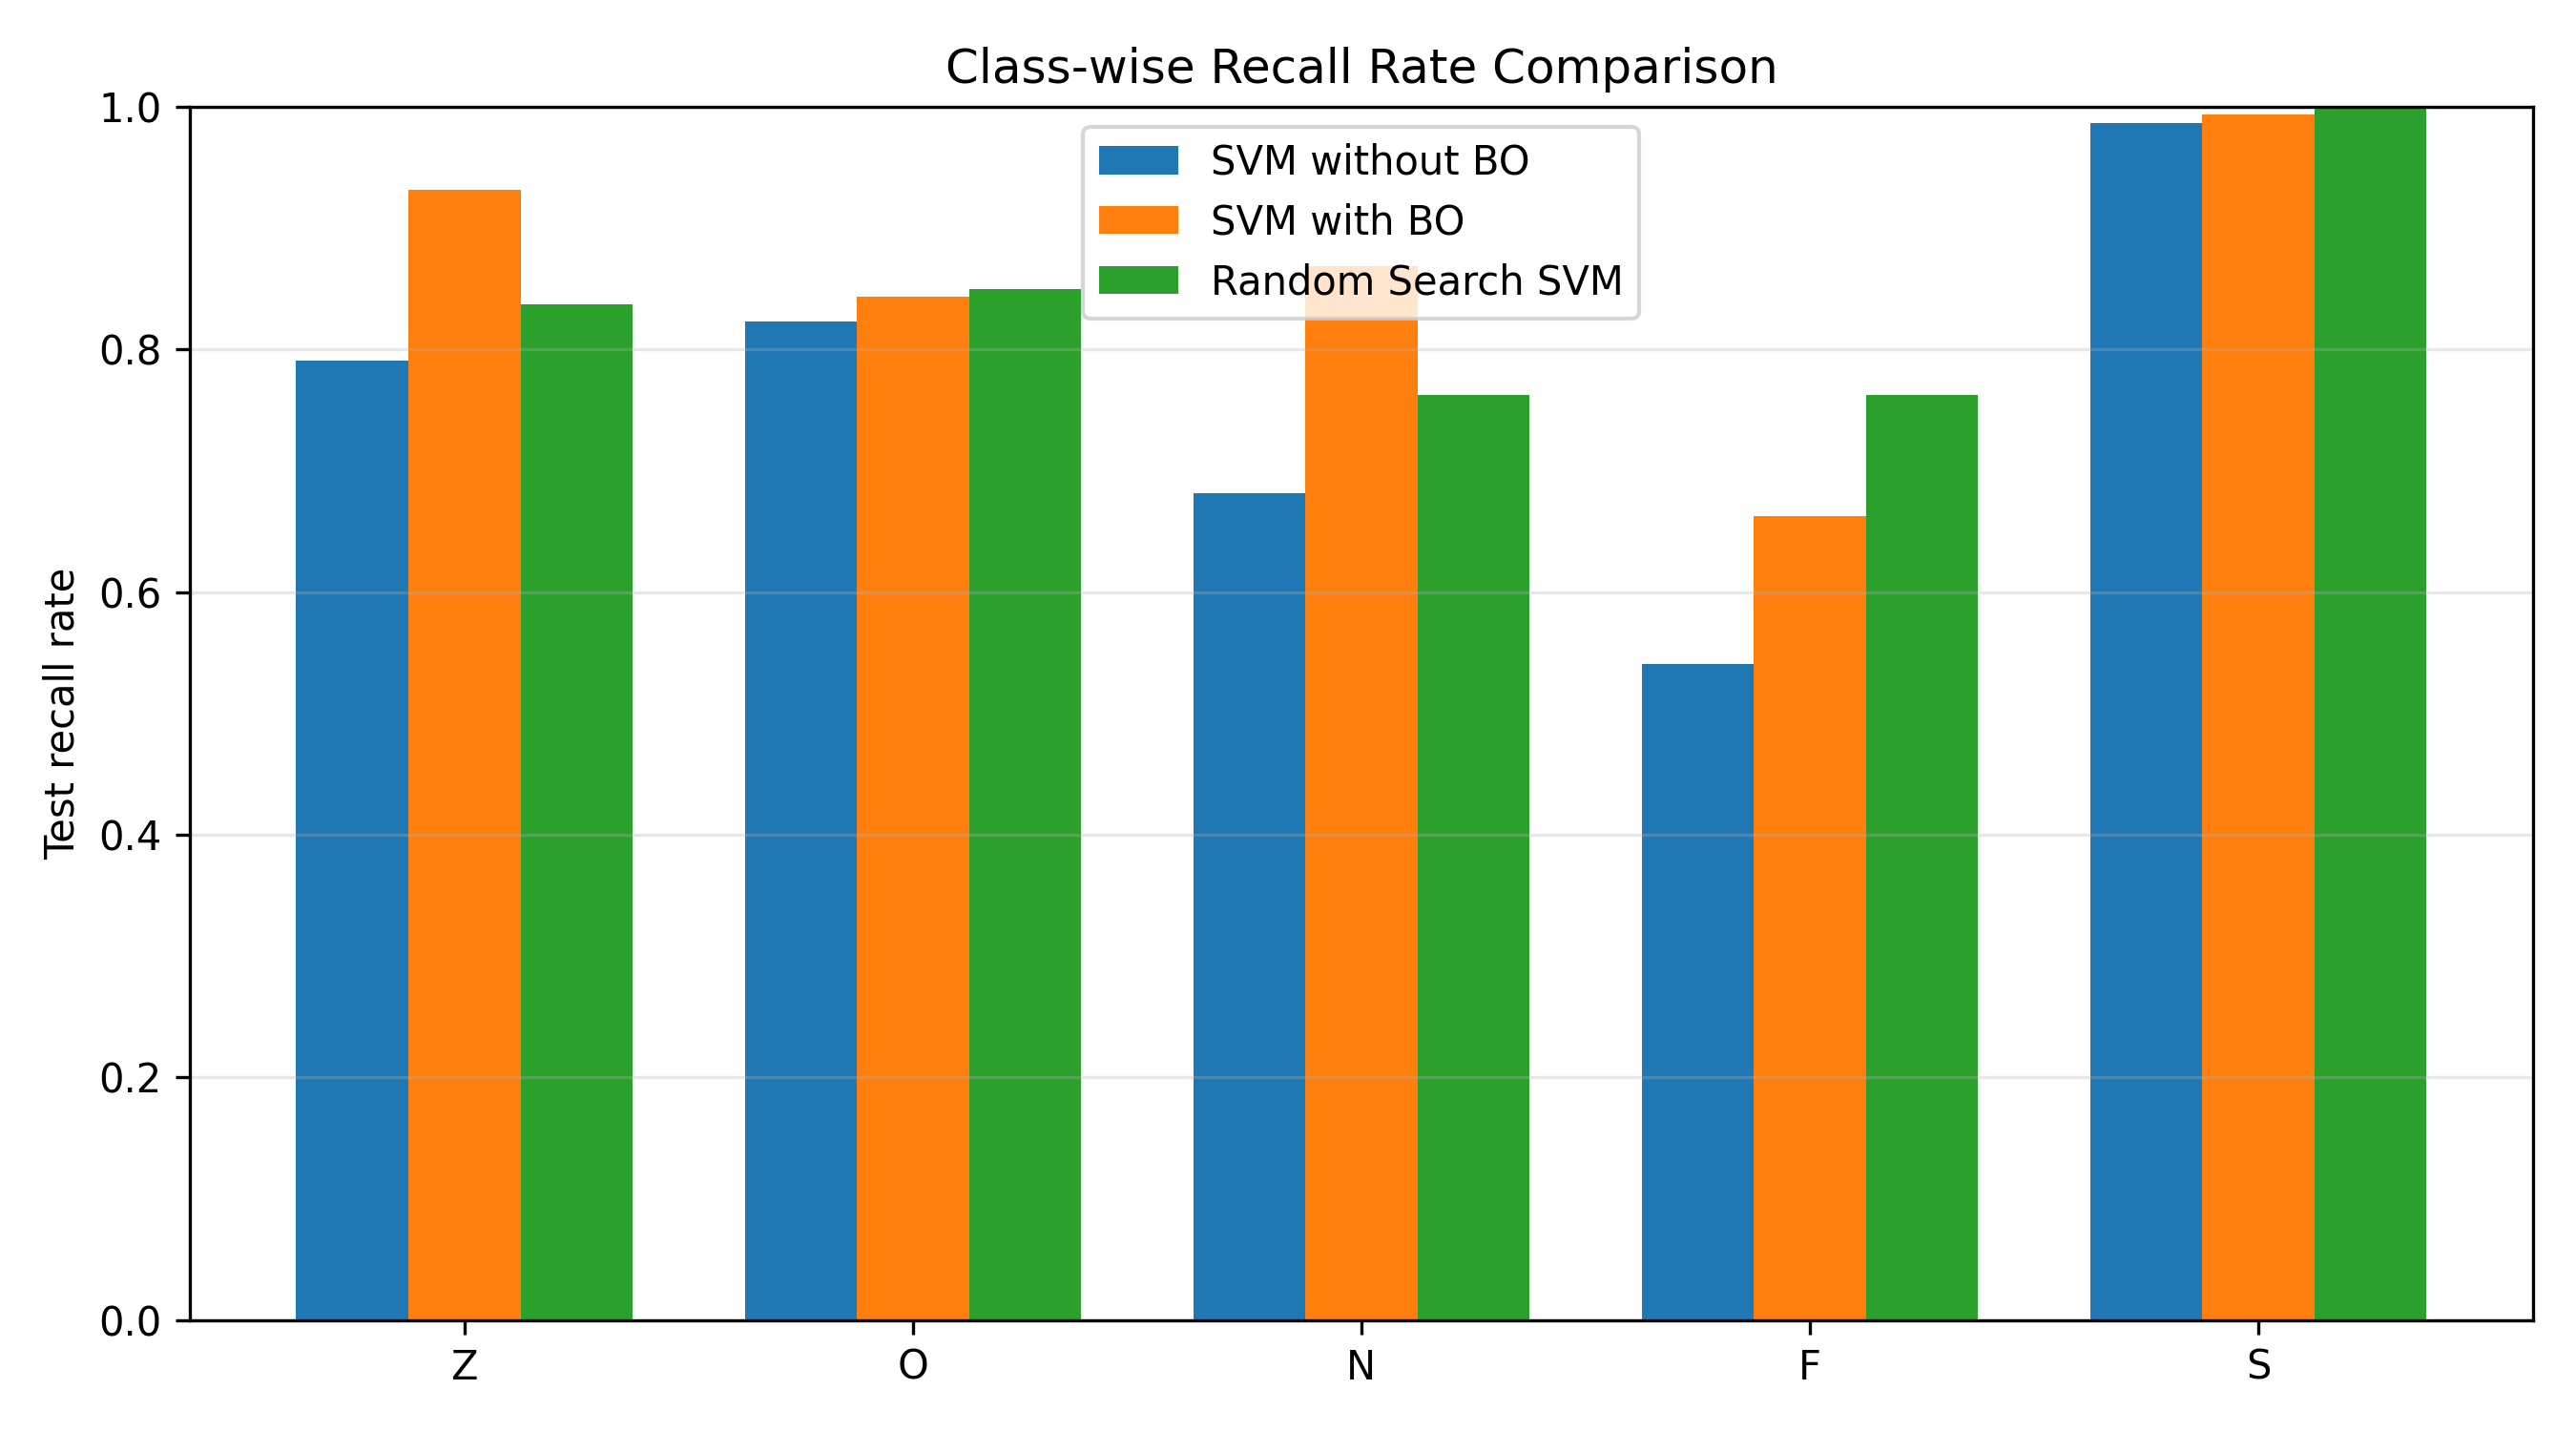
\includegraphics[width=\textwidth]{results/00_main_bo_svm/class_wise_recall_comparison.png}

      \vspace{0.1cm}
      \scriptsize Class-wise recall comparison
    \end{column}

    \begin{column}{0.48\textwidth}
      \centering
      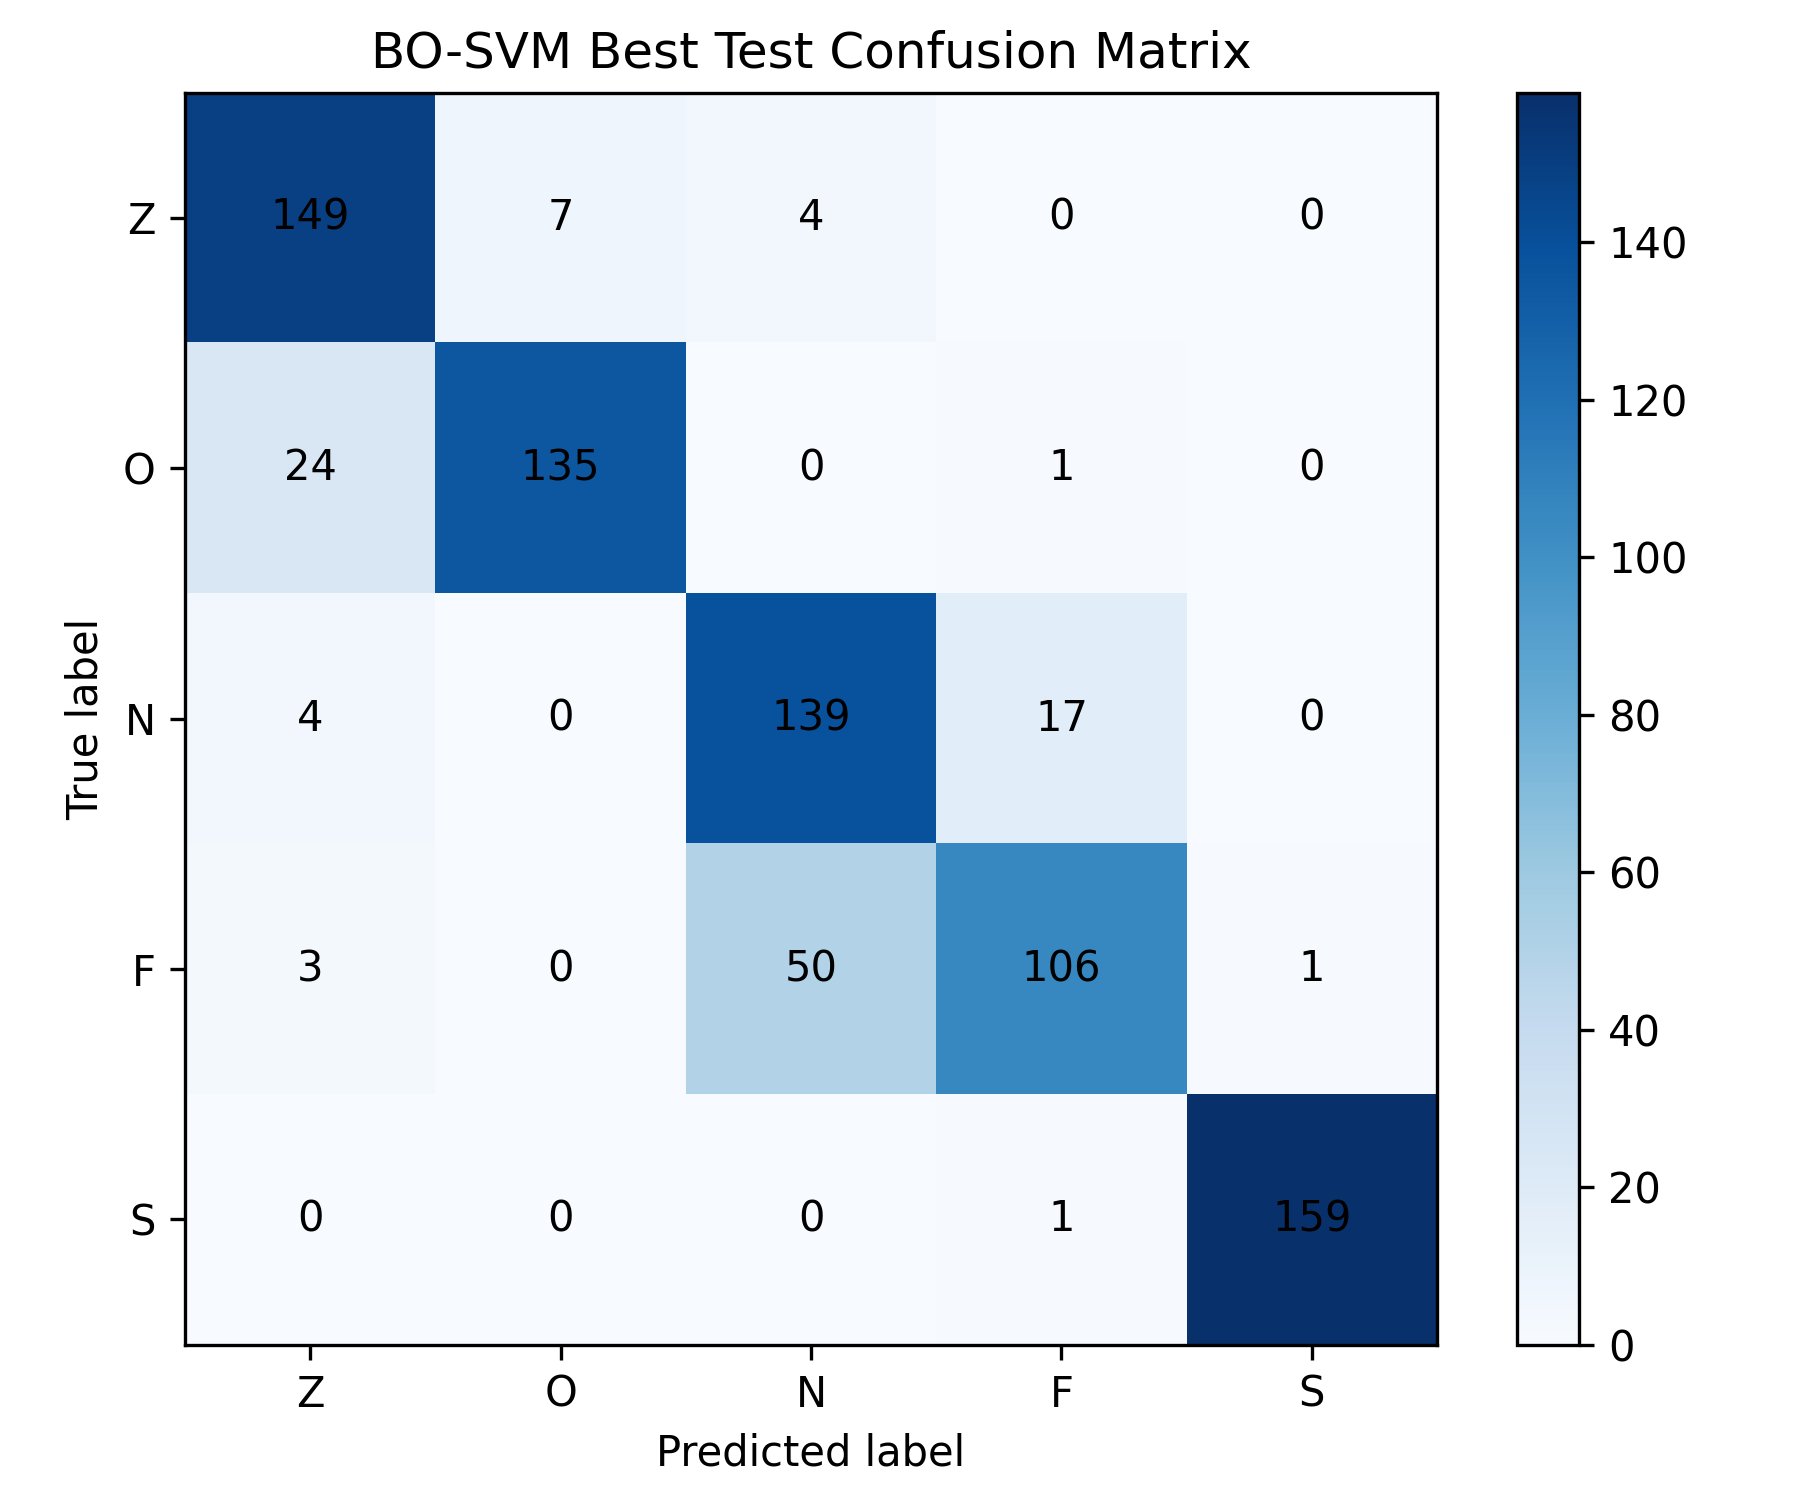
\includegraphics[width=0.92\textwidth]{results/00_main_bo_svm/bo_best_confusion_matrix.png}

      \vspace{0.1cm}
      \scriptsize Best BO-SVM confusion matrix
    \end{column}
  \end{columns}

  \vspace{0.25cm}
  \begin{block}{Observation}
    S was classified very accurately, while the main remaining confusion was between N and F.
  \end{block}
\end{frame}

\begin{frame}{Subset Classification Experiments}
  \begin{itemize}
    \item Binary and three-class Bonn EEG tasks were tested using the full BO-SVM pipeline.
    \item Overlap was included as a BO search parameter for these subset tasks.
    \item These tasks provide reference results for simpler seizure detection settings.
  \end{itemize}

  \begin{table}
    \centering
    \small
    \begin{tabular}{lccc}
      \toprule
      Case & Accuracy & Sensitivity & Specificity \\
      \midrule
      A--E / Z vs S & \textbf{100.00\%} & 100.00\% & 100.00\% \\
      D--E / F vs S & \textbf{98.75\%} & 97.75\% & 99.75\% \\
      A--D--E / Z vs F vs S & \textbf{96.67\%} & 96.67\% & 98.33\% \\
      \bottomrule
    \end{tabular}
  \end{table}
\end{frame}

\begin{frame}{Subset BO Result Visualization}
  \begin{columns}
    \begin{column}{0.48\textwidth}
      \centering
      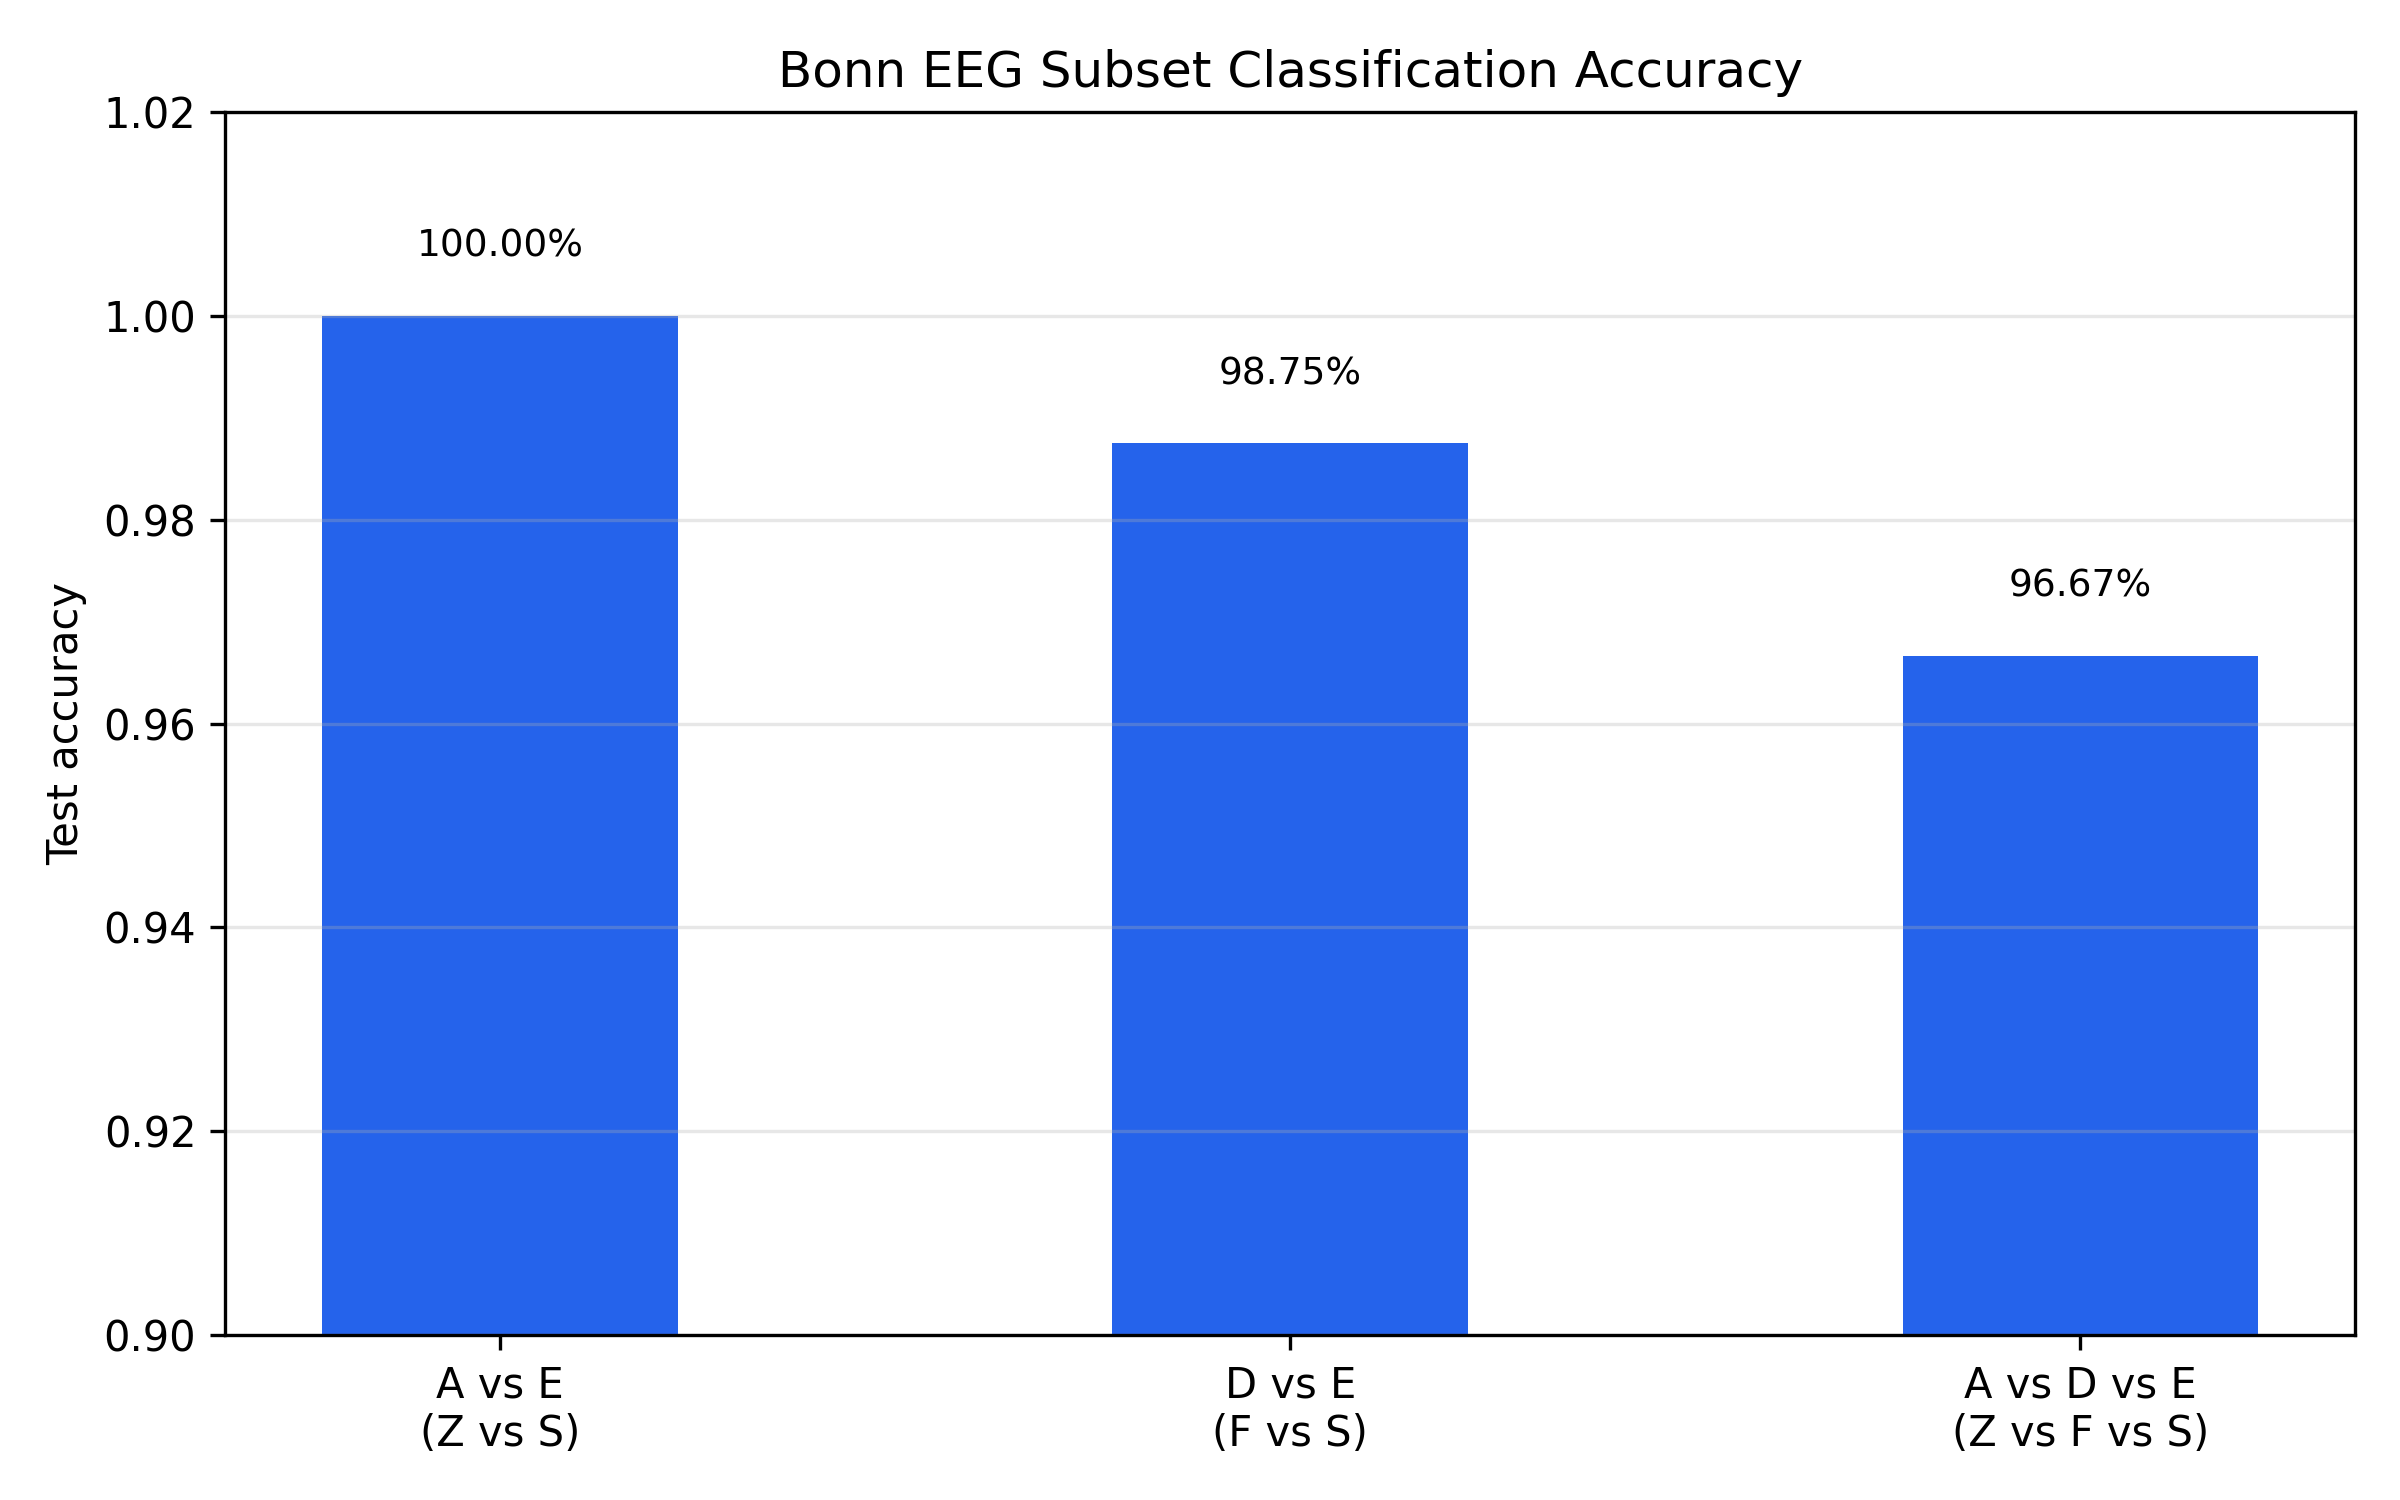
\includegraphics[width=\textwidth]{results/01_subset_tasks/subset_bo_accuracy.png}

      \vspace{0.1cm}
      \scriptsize Subset task accuracy
    \end{column}

    \begin{column}{0.48\textwidth}
      \centering
      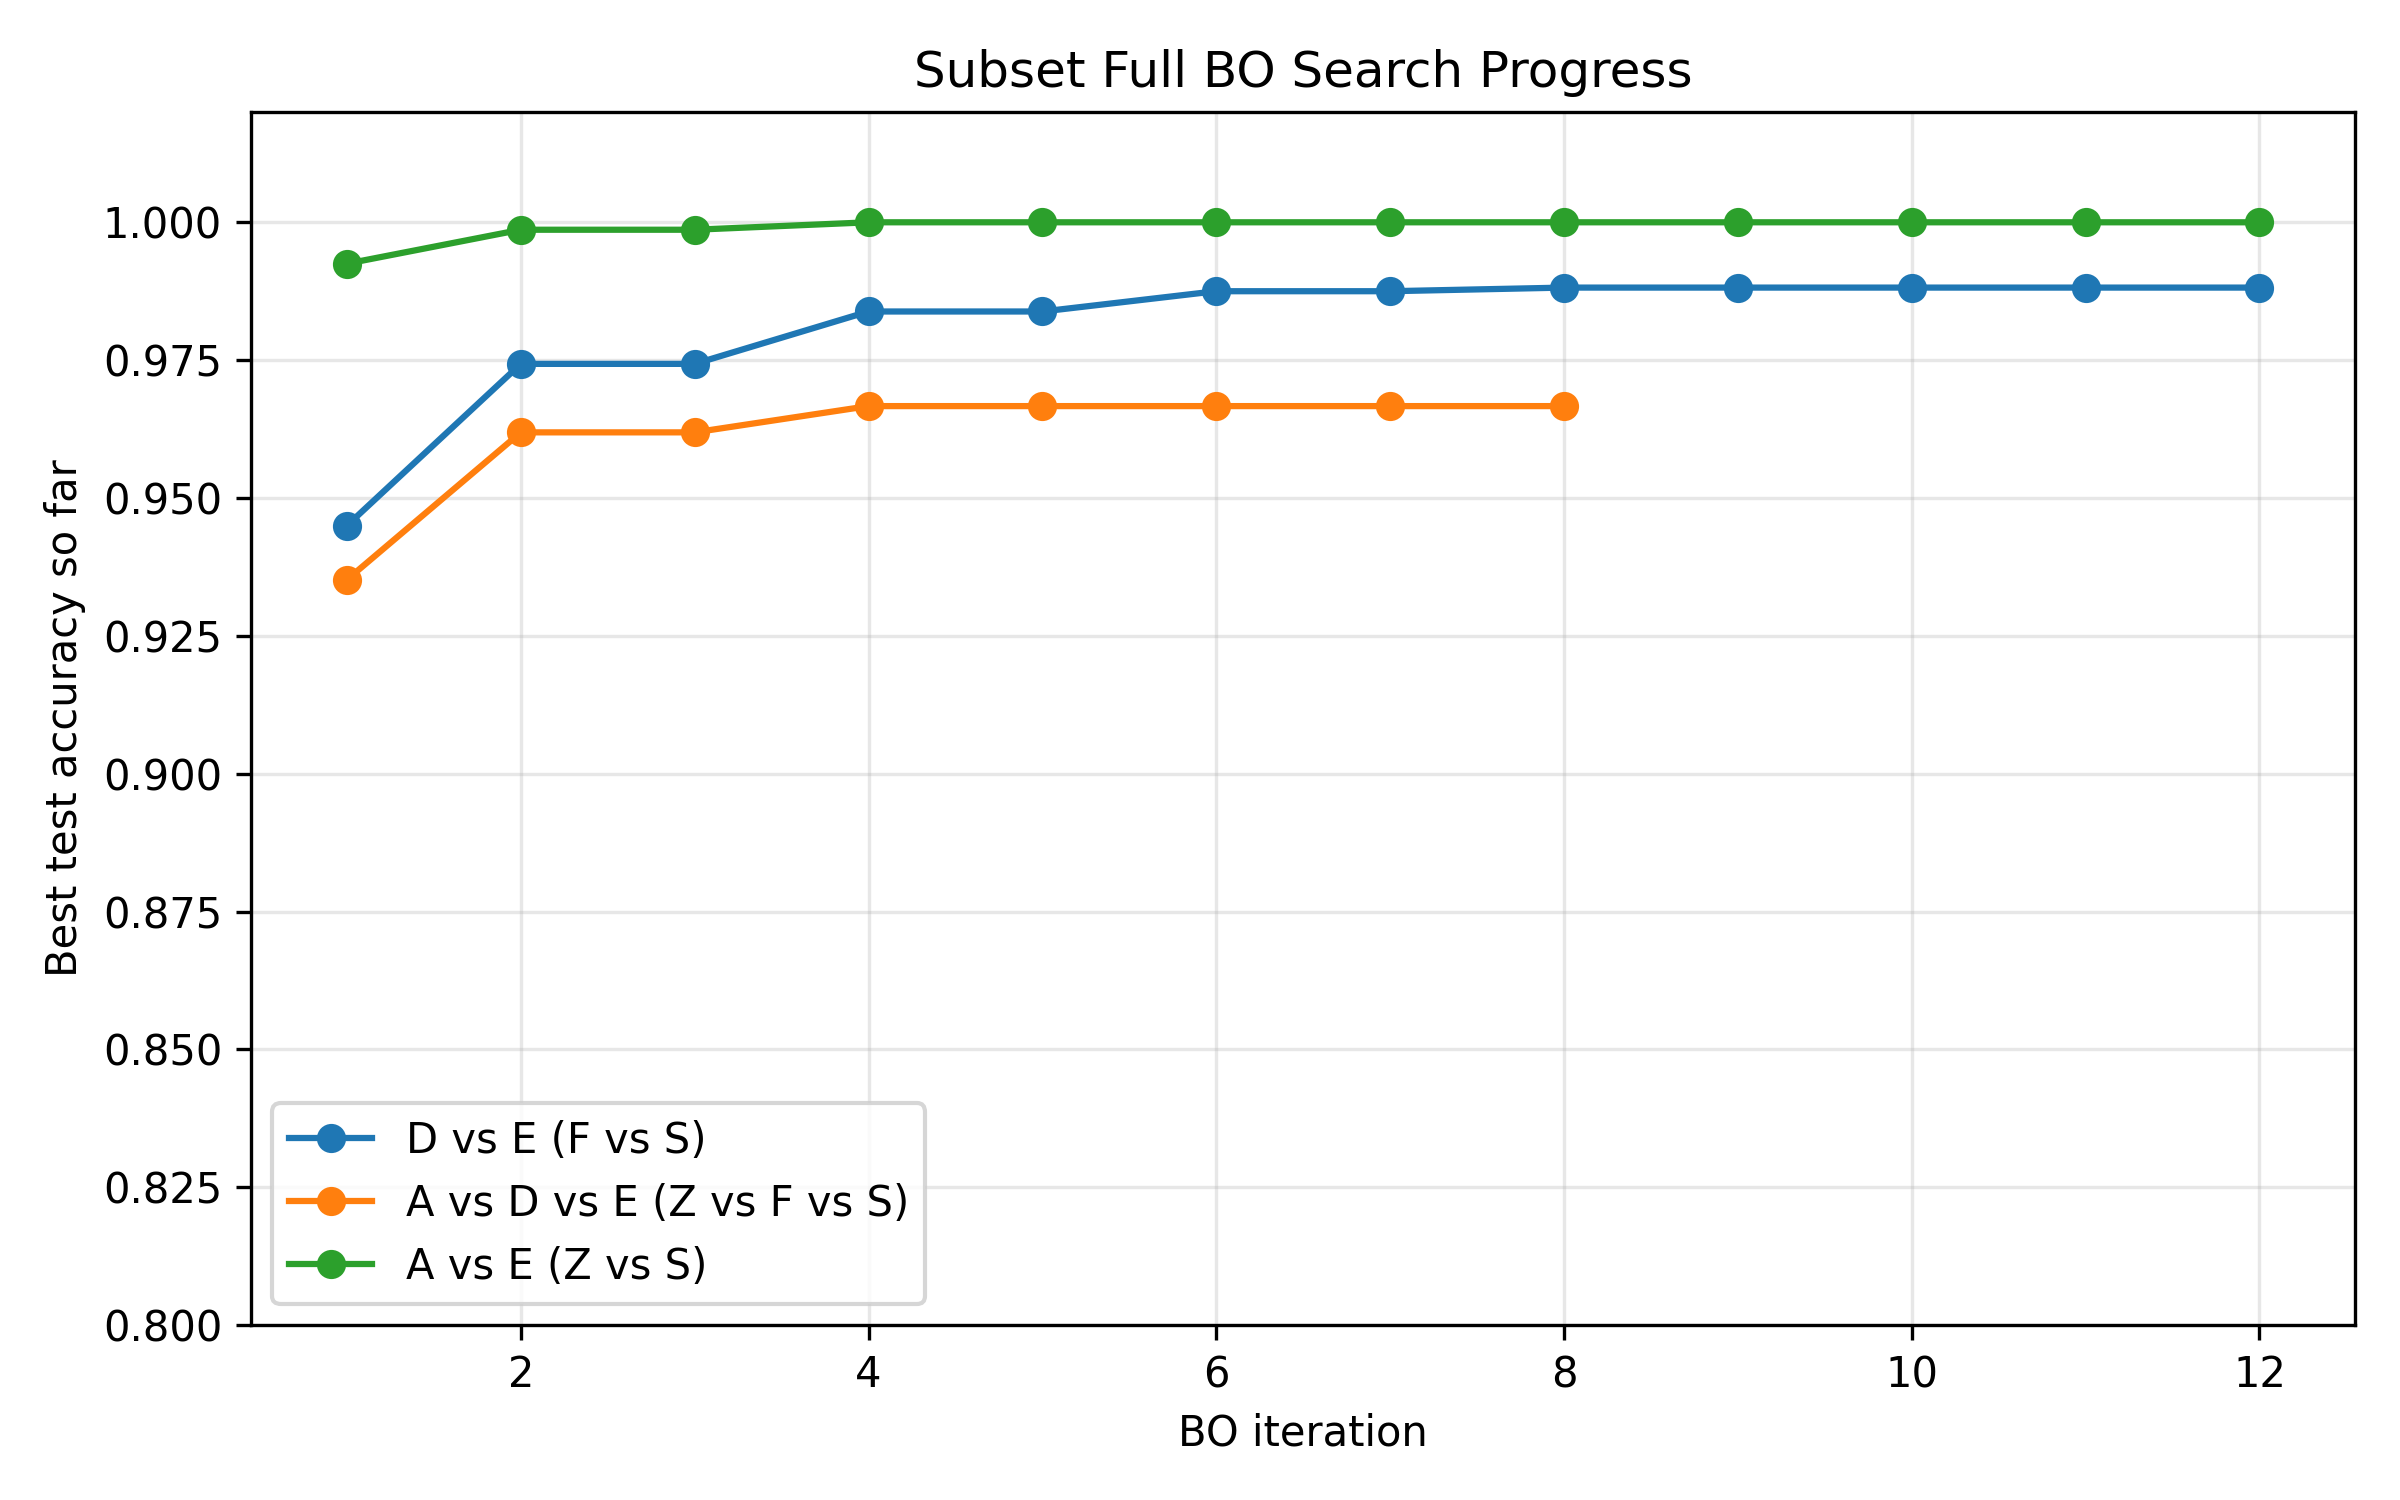
\includegraphics[width=\textwidth]{results/01_subset_tasks/subset_bo_convergence.png}

      \vspace{0.1cm}
      \scriptsize Subset BO search progress
    \end{column}
  \end{columns}
\end{frame}

\begin{frame}{Subset Confusion Matrices}
  \begin{columns}
    \begin{column}{0.32\textwidth}
      \centering
      \textbf{Z vs S}

      \vspace{0.1cm}
      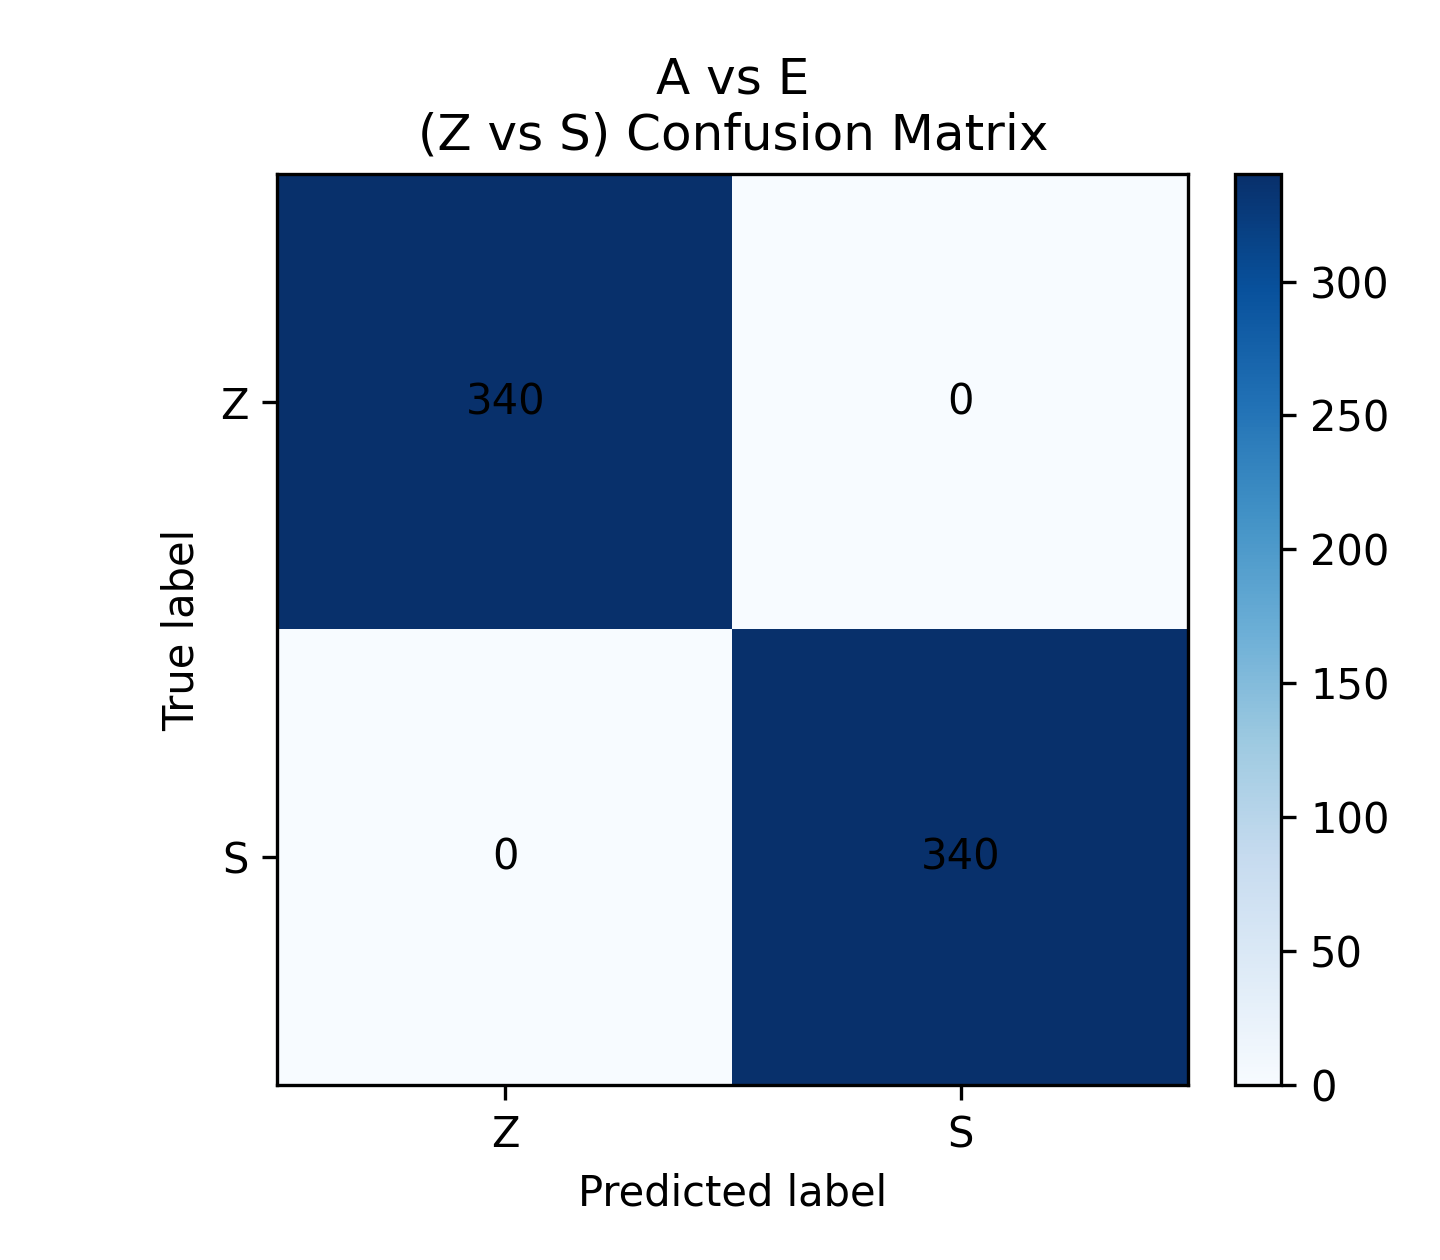
\includegraphics[width=\textwidth]{results/01_subset_tasks/Z_vs_S_confusion_matrix.png}
    \end{column}

    \begin{column}{0.32\textwidth}
      \centering
      \textbf{F vs S}

      \vspace{0.1cm}
      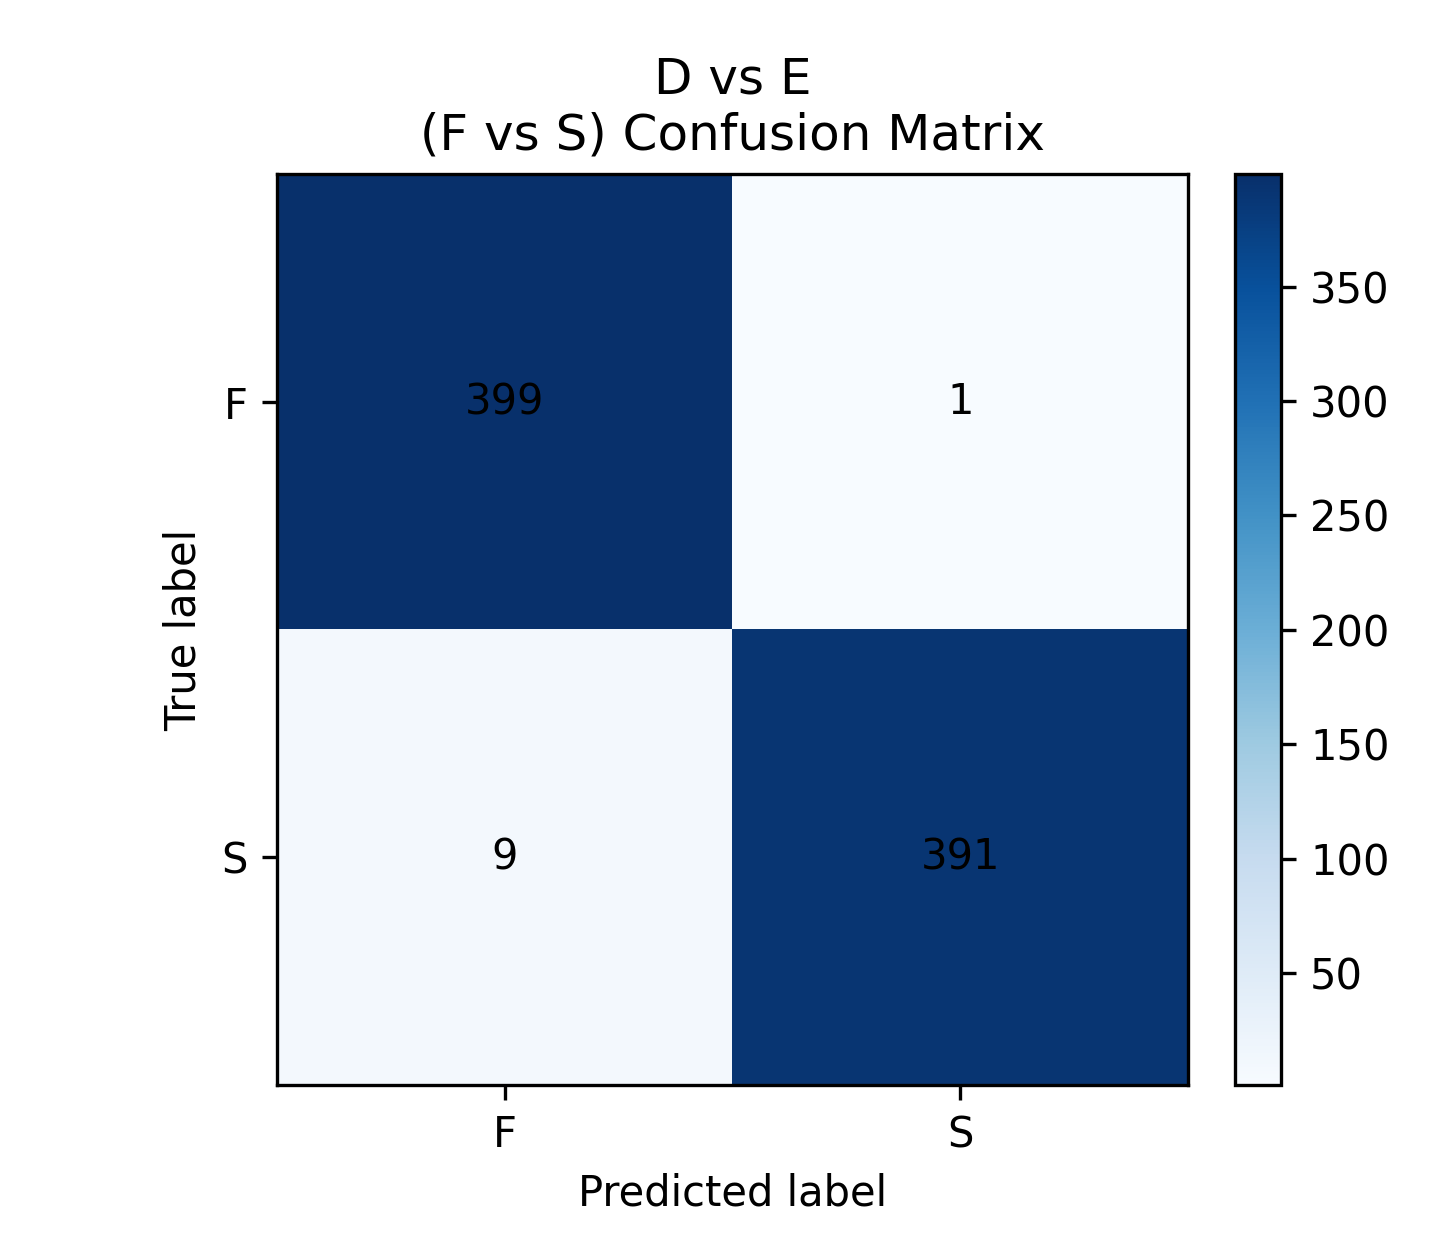
\includegraphics[width=\textwidth]{results/01_subset_tasks/F_vs_S_confusion_matrix.png}
    \end{column}

    \begin{column}{0.32\textwidth}
      \centering
      \textbf{Z vs F vs S}

      \vspace{0.1cm}
      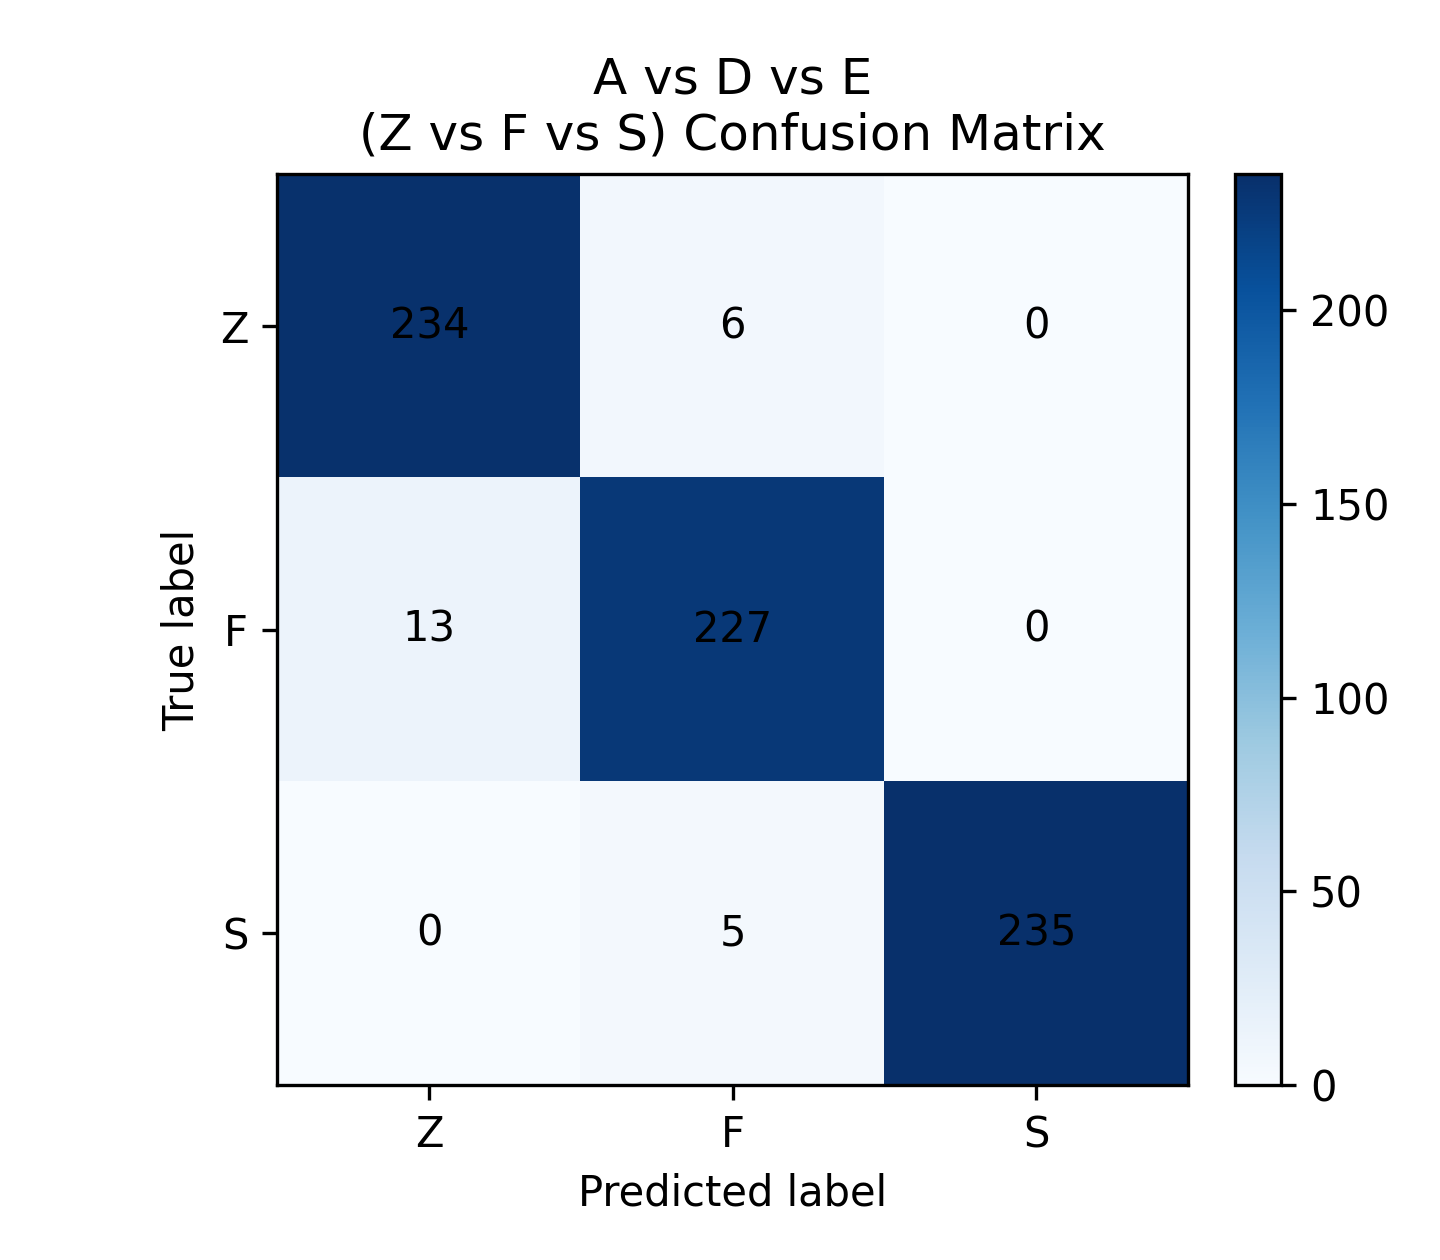
\includegraphics[width=\textwidth]{results/01_subset_tasks/Z_vs_F_vs_S_confusion_matrix.png}
    \end{column}
  \end{columns}

  \vspace{0.45cm}
  \begin{block}{Conclusion From Subset Tasks}
    Binary and three-class tasks reached higher accuracy because they are simpler than complete five-class classification.
  \end{block}
\end{frame}

\section{Discussion and Conclusion}

\begin{frame}{Related Work Reference}
  \begin{table}
    \centering
    \scriptsize
    \begin{tabular}{p{2.6cm}p{3.9cm}p{2.7cm}p{2.2cm}}
      \toprule
      Study / Method & Dataset Setting & Classifier / Technique & Reported Result \\
      \midrule
      Subasi et al. & Bonn dataset & PCA/ICA/LDA + SVM & 100\% accuracy with LDA \\
      Ping Tan et al. & Bonn dataset & Dimensionality reduction + SVM/KNN/DA & 95.00\%, 93.57\%, 94.29\% \\
      Priyanka et al. & Bonn dataset & Artificial Neural Network & 96.9\% accuracy \\
      Guharoy et al. & A--E binary task & ICA with ML classifiers & 100\% for A--E case \\
      This project & Z/O/N/F/S five-class task & Direct BO-SVM & 86.00\% accuracy \\
      This project & A--E, D--E, A--D--E subset tasks & Full BO-SVM & 96.67--100.00\% accuracy \\
      \bottomrule
    \end{tabular}
  \end{table}

  \begin{block}{Important Note}
    Results are used as references only, because different studies use different class combinations, features, and evaluation settings.
  \end{block}
\end{frame}

\begin{frame}{Comparison With Existing Studies}
  \begin{itemize}
    \item Related EEG seizure classification projects were reviewed for performance comparison.
    \item Many reported 99--100\% results use binary or three-class seizure detection tasks.
    \item Complete five-class Bonn EEG classification is more challenging.
    \item Some deep learning methods can report higher five-class performance.
    \item This project uses a lightweight and interpretable feature-based SVM approach.
  \end{itemize}

  \begin{block}{Position of This Work}
    The direct BO-SVM achieved 86.00\% on the five-class task and 96.67--100.00\% on subset tasks, which is reasonable for a handcrafted SVM pipeline.
  \end{block}
\end{frame}

\begin{frame}{Discussion}
  \begin{columns}
    \begin{column}{0.48\textwidth}
      \begin{block}{Advantages}
        \begin{itemize}
          \item Lightweight model
          \item Interpretable features
          \item BO-supported parameter tuning
          \item Overlap included in BO search
          \item Strong subset classification performance
        \end{itemize}
      \end{block}
    \end{column}

    \begin{column}{0.48\textwidth}
      \begin{block}{Limitations}
        \begin{itemize}
          \item Main evaluation is window-level
          \item Overlapping windows may increase train-test similarity
          \item File-level split should be tested in future work
          \item F class recall is still lower than other classes
        \end{itemize}
      \end{block}
    \end{column}
  \end{columns}
\end{frame}

\begin{frame}{Conclusion}
  \begin{itemize}
    \item A complete BO-SVM pipeline was developed for Bonn EEG classification.
    \item BO was run for 80 iterations to tune preprocessing and SVM parameters.
    \item Five-class accuracy improved from 76.45\% to 86.00\% compared with manual SVM.
    \item Binary/three-class subset tasks achieved 96.67--100.00\% accuracy.
    \item Related project comparison showed that subset tasks are usually much easier than full five-class classification.
  \end{itemize}

  \begin{block}{Final Statement}
    The project demonstrates that Bayesian Optimization can improve a lightweight and interpretable SVM-based EEG classification pipeline.
  \end{block}
\end{frame}

\appendix
\section{Backup Slides}

\begin{frame}{Backup: Why SVM?}
  \begin{itemize}
    \item The Bonn dataset is relatively small.
    \item SVM works well with small-to-medium datasets and handcrafted features.
    \item RBF-SVM can model nonlinear decision boundaries.
    \item Compared with deep learning, SVM is more lightweight and interpretable.
  \end{itemize}
\end{frame}

\begin{frame}{Backup: Why Bayesian Optimization?}
  \begin{itemize}
    \item Manual parameter selection may miss better combinations.
    \item Random Search does not use previous trial results to guide the next trial.
    \item BO builds a surrogate model of the objective function.
    \item It searches preprocessing and SVM hyperparameters more systematically.
  \end{itemize}
\end{frame}

\begin{frame}{Backup: What Does Window-Level Mean?}
  \begin{itemize}
    \item Each original EEG segment is divided into smaller windows.
    \item Classification is performed at the window level.
    \item With overlapping windows, neighboring windows share part of the signal.
    \item Therefore, the 86.00\% five-class BO-SVM result should be described as window-level accuracy.
  \end{itemize}
\end{frame}

\begin{frame}{Thank You}
  \centering
  \Huge Thank You

  \vspace{0.6cm}
  \Large Questions?
\end{frame}

\end{document}
